\documentclass[letter]{article}
\renewcommand{\baselinestretch}{1.25}

\usepackage[margin=1in]{geometry}
\usepackage{physics}
\usepackage{amsmath, mathtools}
\numberwithin{equation}{section}
\usepackage{amssymb}
\usepackage{graphicx}
\usepackage{hyperref}
\usepackage{empheq}

% MATLAB Formating Code
\usepackage[numbered,framed]{matlab-prettifier}
\lstset{style=Matlab-editor,columns=fullflexible}
\renewcommand{\lstlistingname}{Script}
\newcommand{\scriptname}{\lstlistingname}

\allowdisplaybreaks

%opening
\title{MECH 6323 - HW 1}
\author{Jonas Wagner}
\date{2022, January 24}

\begin{document}	

\maketitle

% \tableofcontents

%----------------------------------------------------------------------------
% \newpage
\section{Problem 1}









\newpage
\section{Problem 3}
\textbf{Problem:}
For each of the bode plots:
\begin{enumerate}
	\item Determine the breakpoints and the transfer function.
	\item Determine the gain cross-over frequency $\omega_c$ and the phase cross-over frequency $\omega_{180}$.
\end{enumerate}

\subsection{Bode Plot 1:}
\begin{figure}[h]
	\centering
	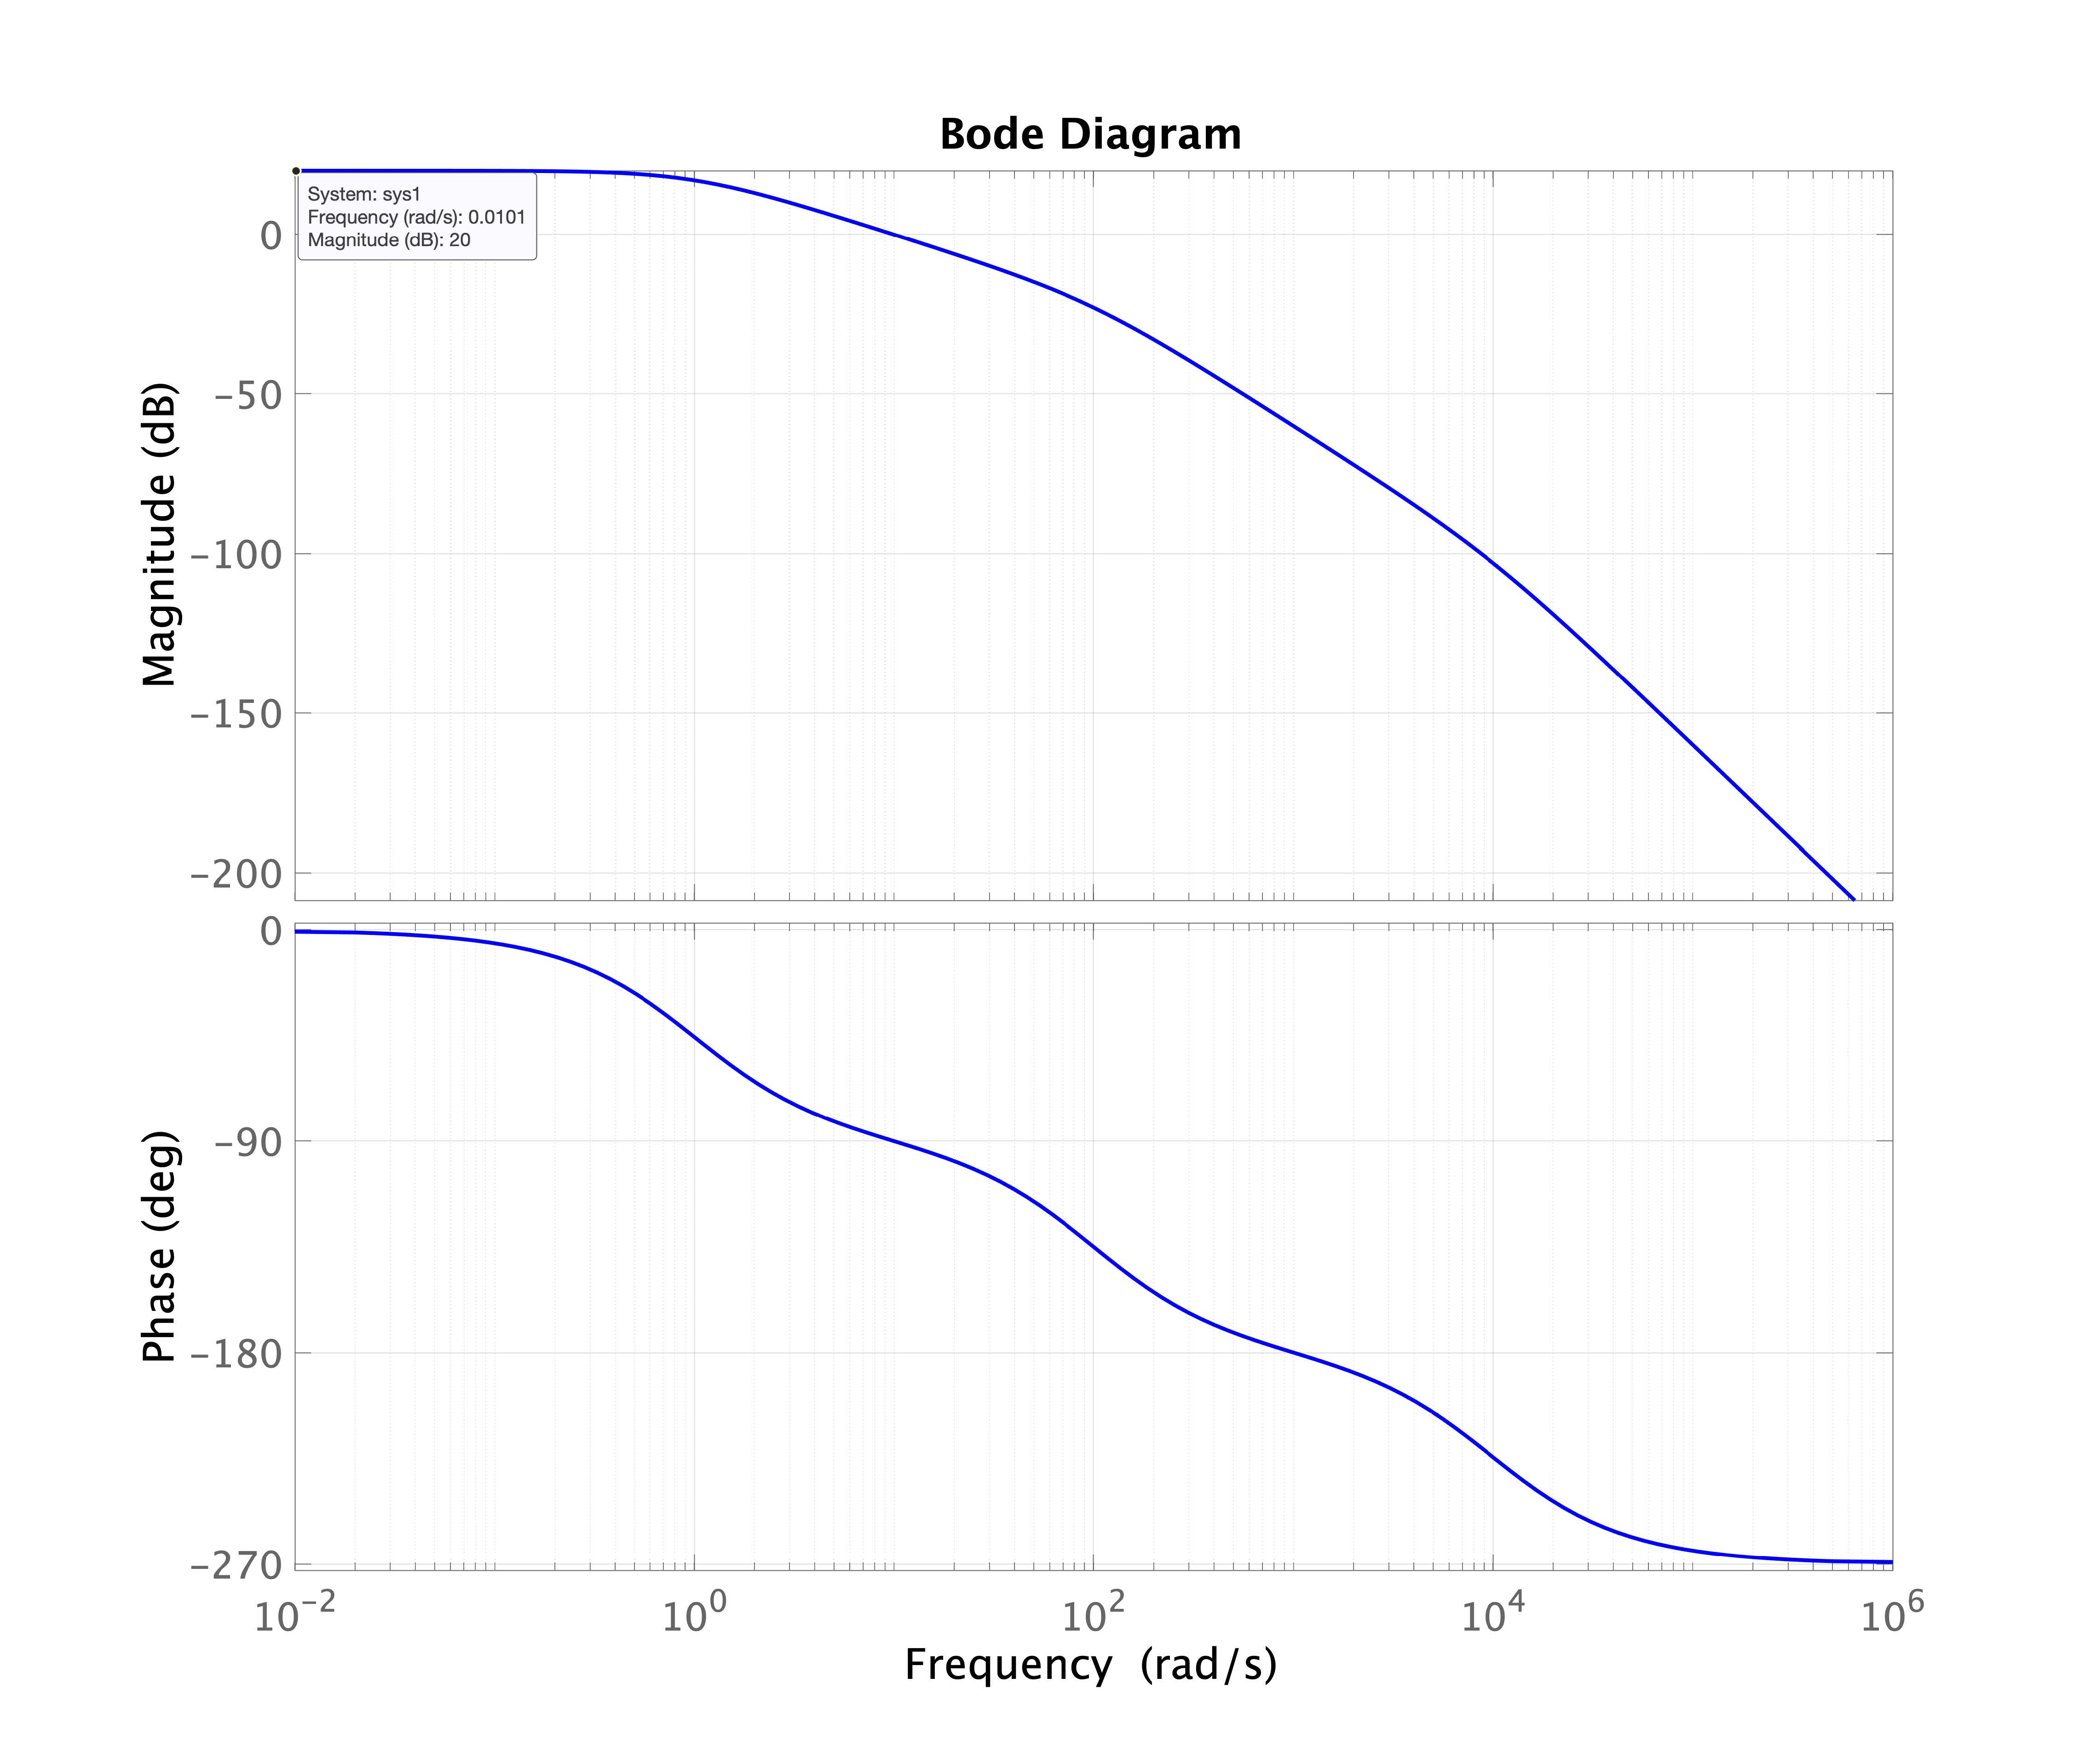
\includegraphics[width=0.5\textwidth]{figs/pblm3a.jpg}
\end{figure}

\textbf{Gain, Poles, and Zeros:}
\begin{enumerate}
	\item \textbf{Gain:}  $20$ db = 10
	\item \textbf{Poles:}
	\begin{enumerate}
		\item $10^{0} = 1$ rad/s
		\item $10^{2} = 100$ rad/s
		\item $10^{4} = 10,000$ rad/s
	\end{enumerate}
	\item Zeros: (NA)
\end{enumerate}

\textbf{Transfer Function:}\[
	H(s) = \cfrac{10}{
		\qty(1 + \frac{s}{1}) \qty(1 + \frac{s}{100}) \qty(1 + \frac{s}{10000})
		}
\]

\textbf{Cross-over Frequency:}
\begin{enumerate}
	\item $\omega_c = 10^{1} = 10$ rad/s
	\item $\omega_{180} = 10^{3} = 100$ rad/s
\end{enumerate}



\newpage
\subsection{Bode Plot 2:}
\begin{figure}[h]
	\centering
	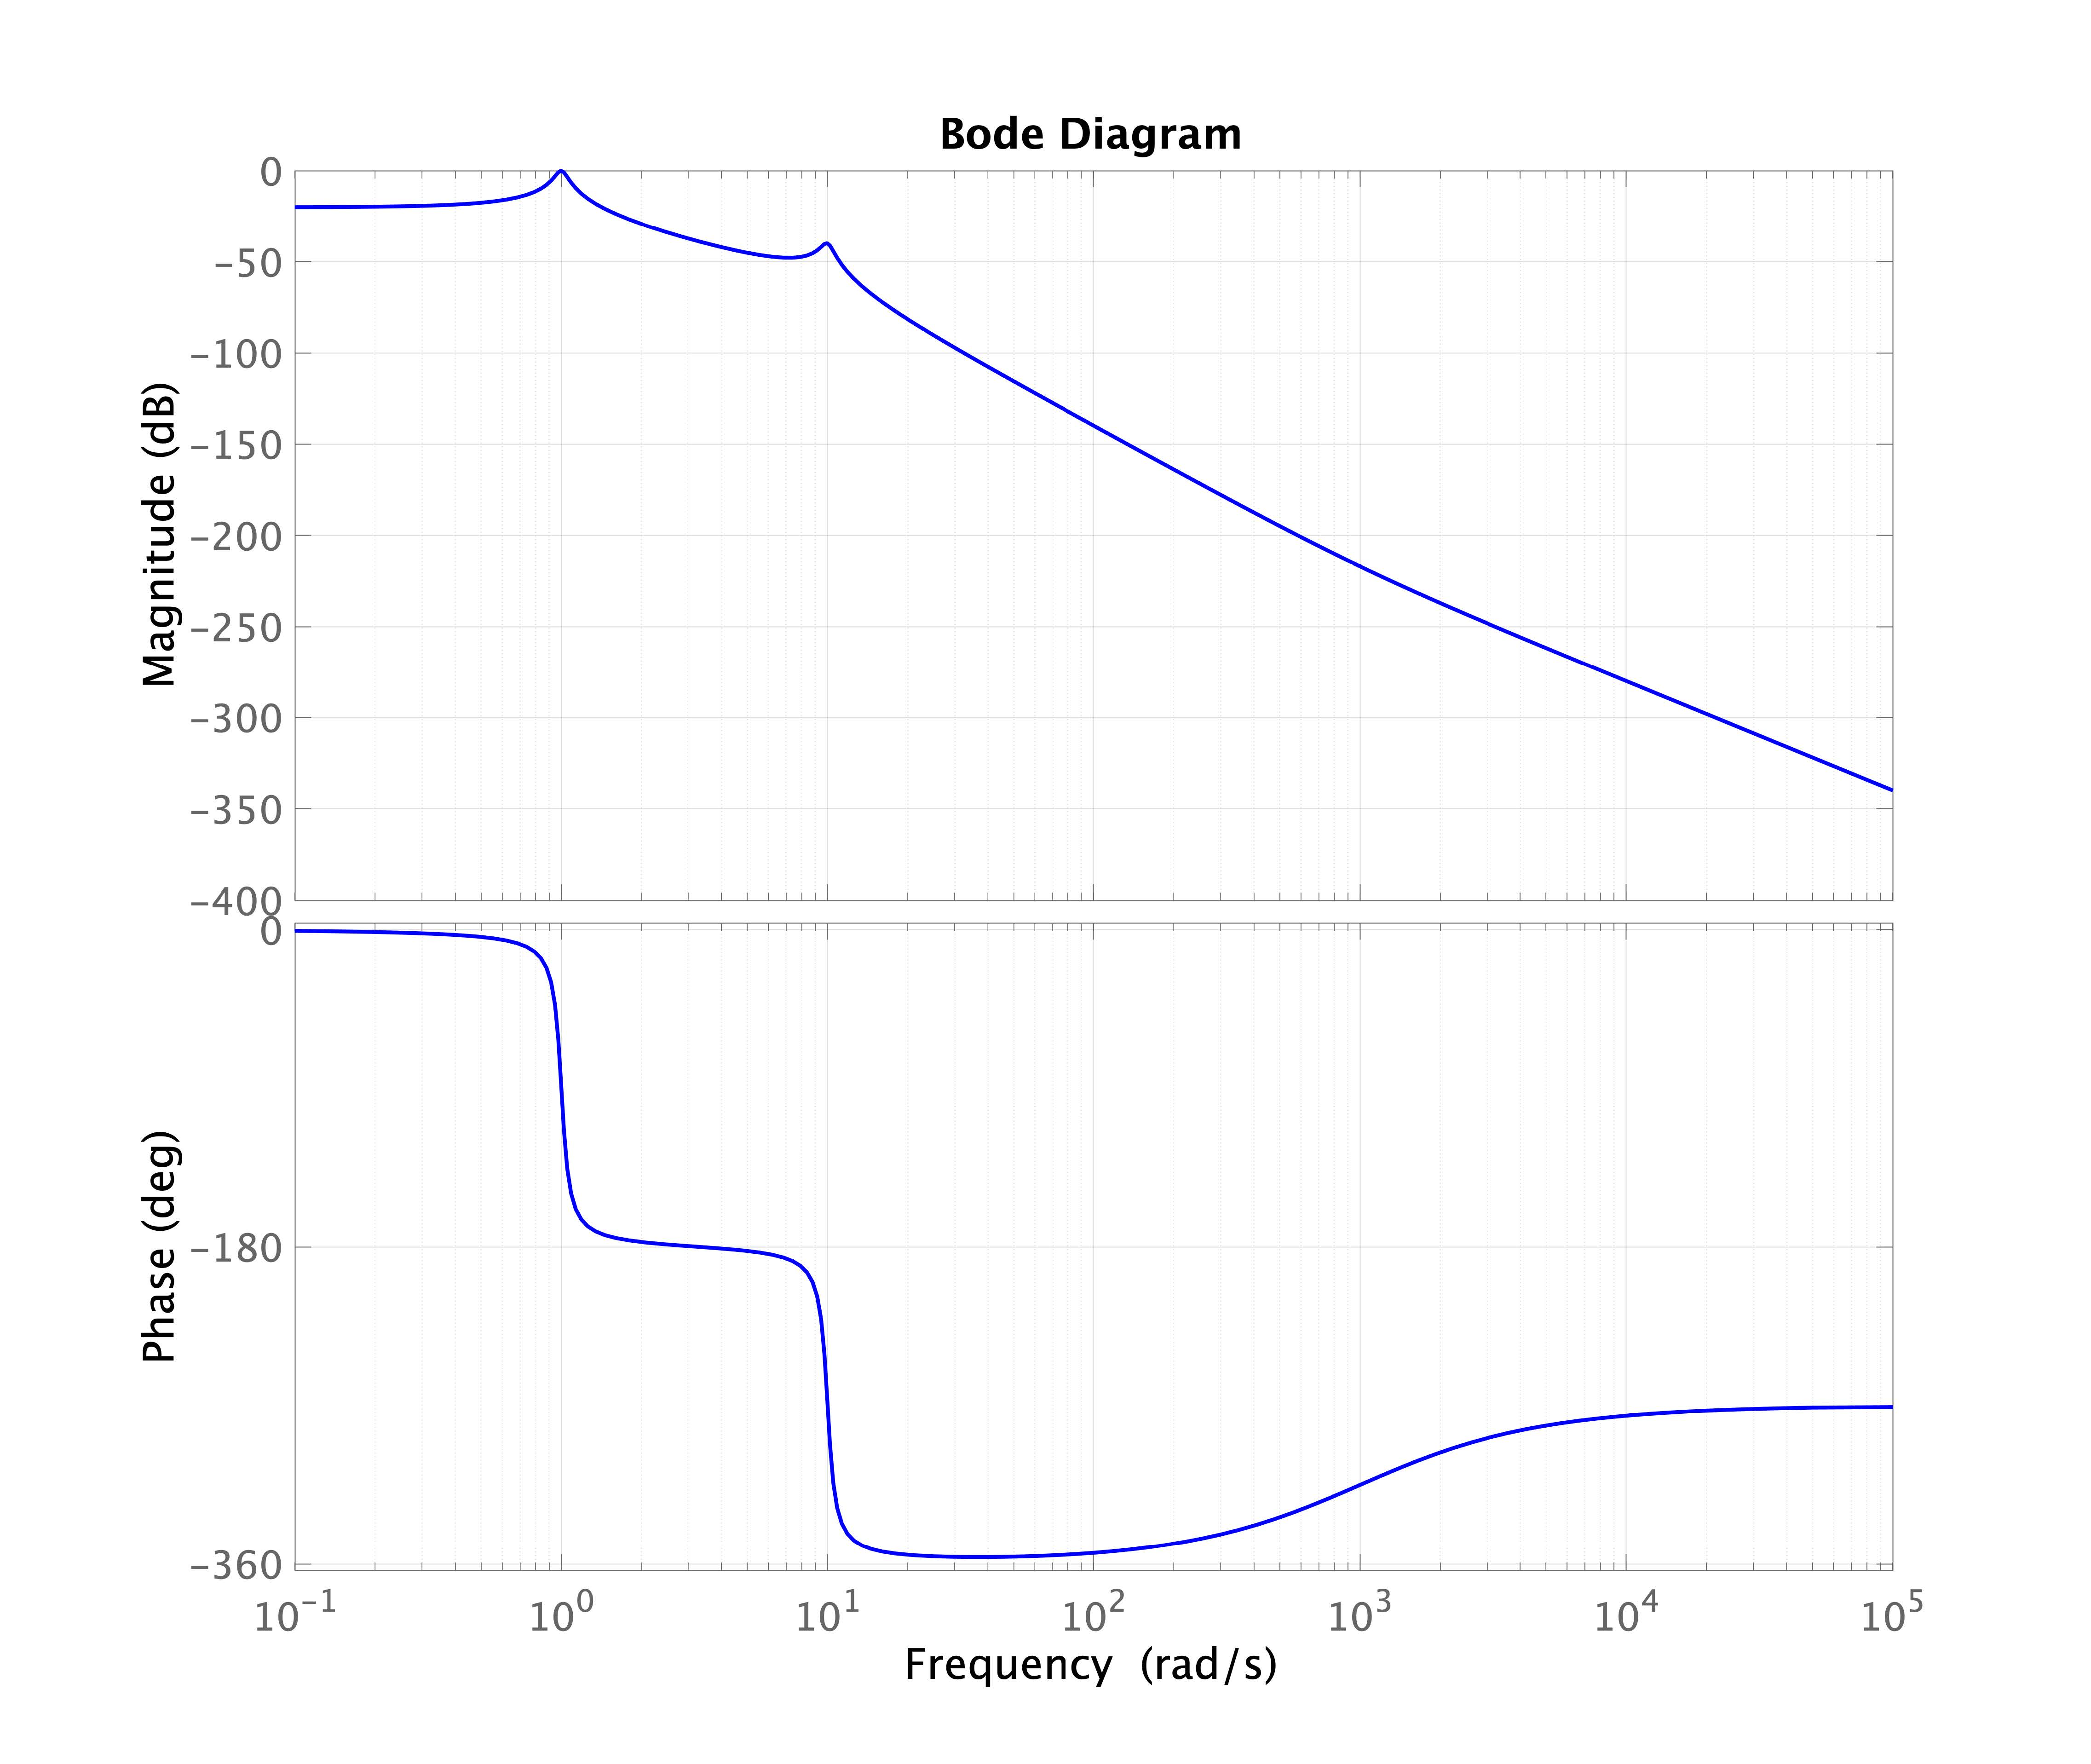
\includegraphics[width=0.5\textwidth]{figs/pblm3b.jpg}
	\caption{Bode Plot 2}
\end{figure}

\textbf{Gain, Poles, and Zeros:}
\begin{enumerate}
	\item \textbf{Gain:}  $20$ db = 10
	\item \textbf{Poles:}
	\begin{enumerate}
		\item $10^{0} = 1$ rad/s
		\item $10^{2} = 100$ rad/s
		\item $10^{4} = 10,000$ rad/s
	\end{enumerate}
	\item Zeros: (NA)
\end{enumerate}

\textbf{Transfer Function:}\[
	H(s) = \cfrac{10}{
		\qty(1 + \frac{s}{1}) \qty(1 + \frac{s}{100}) \qty(1 + \frac{s}{10000})
		}
\]


% \newpage
% \appendix
% \section{MATLAB Code:}\label{apx:matlab}
% All code I write in this course can be found on my GitHub repository:\\
% \href{https://github.com/jonaswagner2826/MECH6313}{https://github.com/jonaswagner2826/MECH6313}


\end{document}
